\begin{figure}[h!]
  \begin{center}
    \caption{Graph of Fitness Function}
    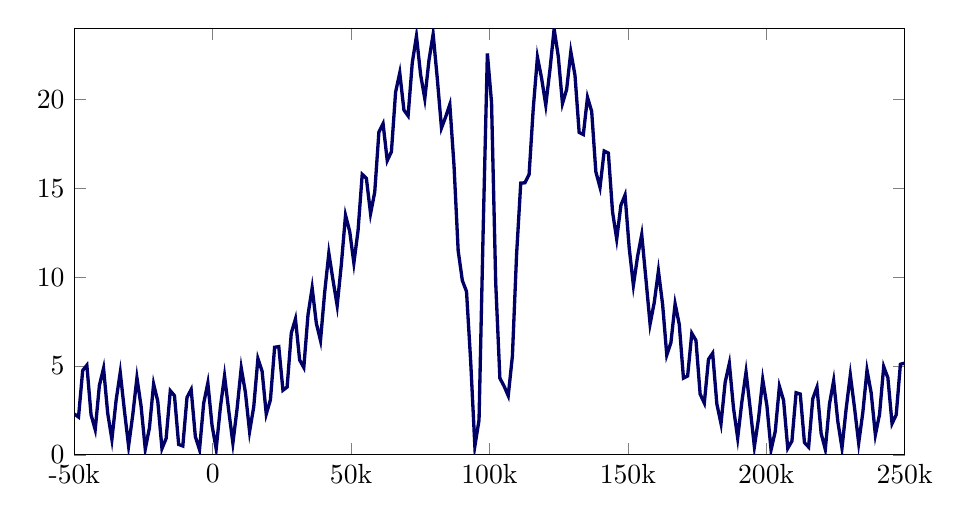
\begin{tikzpicture}
      \begin{axis}[
          xmin=-50000,
          xmax=250000,
          scaled x ticks=false,
          xtick={-50000,0,50000,100000,150000,200000,250000},
          xticklabels={-50k,0,50k,100k,150k,200k,250k},,
          ymin=0,
          ymax=24,
          width=\textwidth,
          height=7cm,
        ] \addplot[
          no marks,
          very thick,
          blue!40!black,
          % <->
        ] expression[
          domain=-50000:250000,
          % samples=3000
          samples=200
        ]{12+10*(cos(deg(ln(0.1+(0.001*x-100)^2))))-(2*sin(deg(0.001*x-100)))};
      \end{axis}
    \end{tikzpicture}
  \end{center}
\end{figure}
